\documentclass[12pt,a4paper]{article}
\usepackage{inverba}
\newcommand{\userName}{Cullyn Newman} 
\newcommand{\class}{BI 216} 
\newcommand{\institution}{Portland State University} 
\newcommand{\thetitle}{\hypertarget{home}{Lab 8: Scientific Writing/Reading}}
\rfoot{\hyperlink{home}{\thepage}}
\color{lightmodetext}
\pagecolor{lightmode}
\definecolor{under}{HTML}{9e9e9e}
\begin{document}
\section*{Introduction}
\begin{enumerate}[font=\bfseries, wide]
    {\color{under}\item Your TA will assign your group a topic to learn more about and present to the class. Record notes on your team’s findings/discussion of your specifically assigned topic below. (1 pt)}
    
    \textbf{Assigned Topic:} Population Dynamics Model

    \textbf{Notes:} Homing failure was introduced using it's estimated upper and lower bound into Khoury's et al. poplation model. The simulation used population sizes of 15,000 to 18,000, which are average values estimated by bee keepers. Foragers accounted for 25\% of the total population. Natural death was 0.154 individuals per day. Other factors were kept the same. 

    Hypothesis was constant forager death rate with no forager exposure and forager death rate raised by post-exposure homing failure during a 30-days oilseed rape flowering period. 
    
    {\color{under}\item Insert a picture of your team’s concept map of the introduction below. Use the words in the word bank below. Don’t forget to include linking words between each connection!   (1 pt)}
    
    \begin{center}
        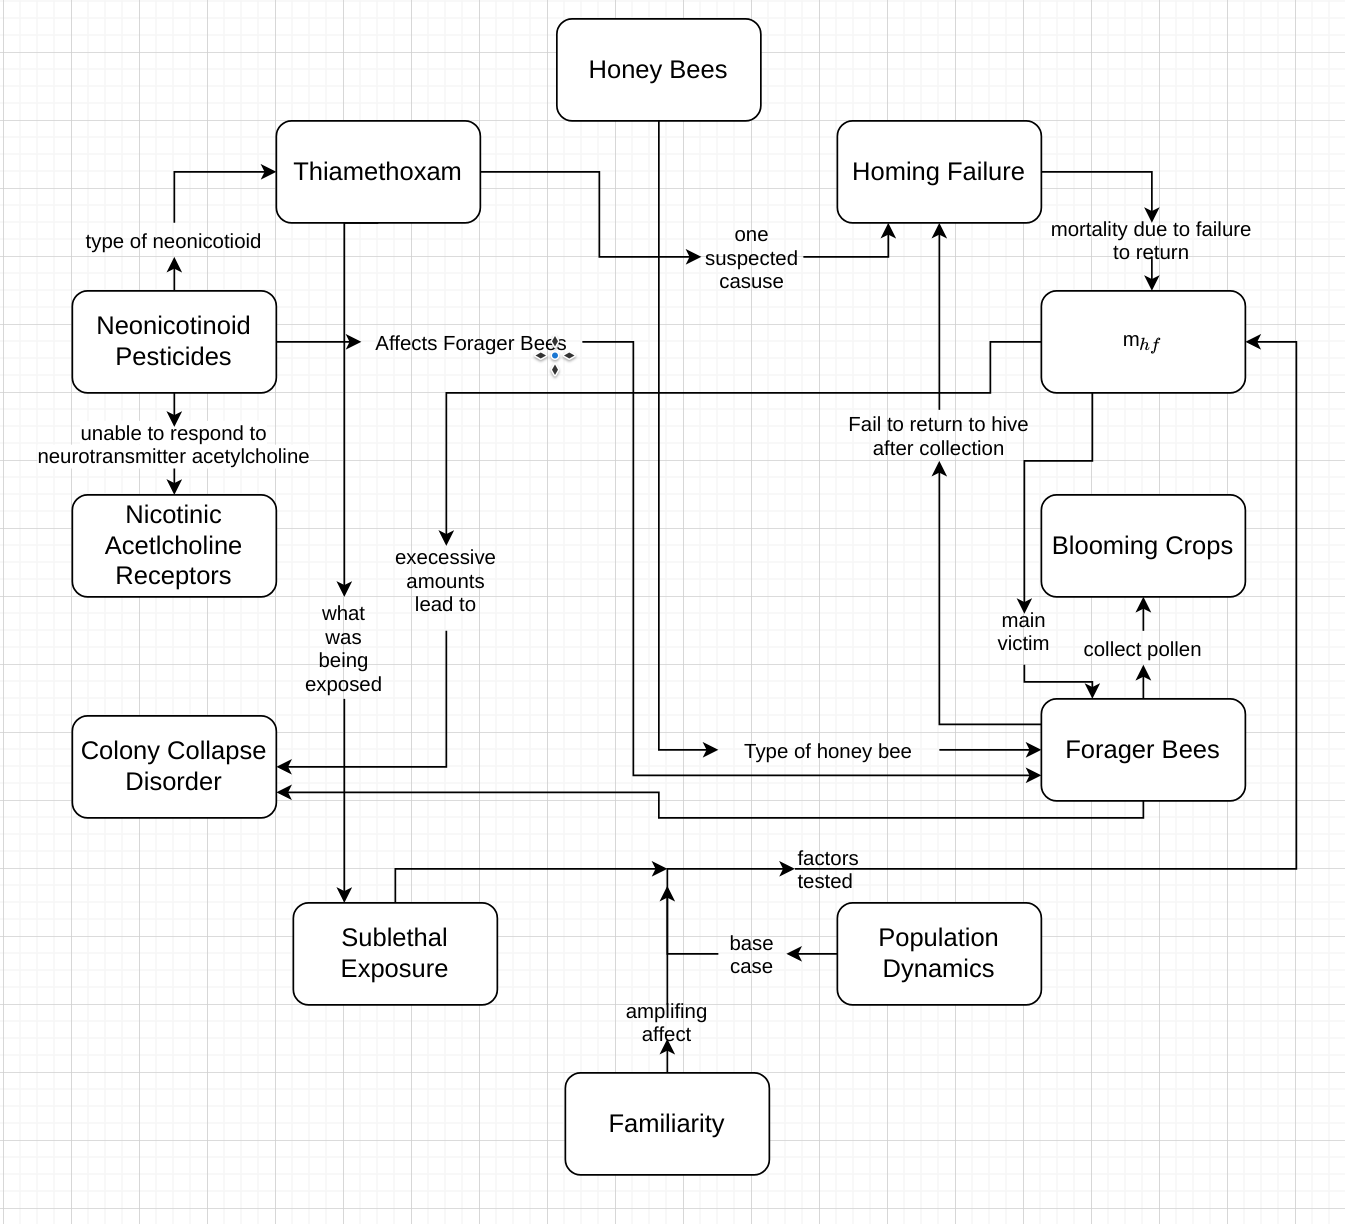
\includegraphics[scale=0.33]{images/map.png}
    \end{center}
    \vspace{-1cm}
    
    
    {\color{under}\item What is the overarching hypothesis that the authors of this study want to test? (1 pt)}
    
    Sublethal exposure to a neonicotinoid (thiamethoxam) indirectly increases hive death rate through homing failure in foraging honey bees.
    
\end{enumerate}

\section*{Methods}
\begin{enumerate}[font=\bfseries, wide, resume]
    {\color{under}\item What is the specific question the authors are attempting to answer with “Experiment 1?” (1 pt)}
    
    They were simulating the intoxication at a \textit{familiar} foraging site. 

    {\color{under}\item What is the specific question the authors are attempting to answer with “Experiment 2?” (1 pt)}

    They were simulating the intoxication at a \textit{random} foraging site, or one they have no familiarity or past forager experience with. 

    {\color{under}\item Insert a picture of your team’s sketch of the methods used to produce Figure 3 below. (1 pt)}
    
    

    {\color{under}\item Insert a picture of your team’s sketch of the methods that would be used to produce Figure 4 below. (1 pt)}
    
    \subsection*{Figure 3 Analysis Questions}
    {\color{under}\item What is the “control” group and what is the “treated” group? (1 pt)}
    
    Treated honey bees are bees that received a nonlethal dose of thiamethoxam. The control group was treated with untreated sucrose solution. 

    {\color{under}\item What do you learn when you compare Panel A to Panel B? (1 pt)}

    Treated bees suffered in both familiar and unfamiliar sites, but bees in unfamiliar sites suffered greater in unfamiliar.

    {\color{under}\item Overall, what do you learn from Figure 3? (1 pt)}
    
    Thiamethoxam may impact learning and memory in bees, or some other function that allows them to find their way back, as bees in unfamiliar sites seem more impacted. 

    \subsection*{Figure 4 Analysis Questions}
    {\color{under}\item  What do the two sets of red and blue lines in each of the graphs in this figure represent? (1 pt)}
    
    Red lines: population dynamics between simulated colonies exposed to thiamethoxam. Blue lines were not exposed.

    {\color{under}\item What do the grey shaded areas represent? (1 pt)}
    
    The exposue period to nonlethal thiamethoxam.
    
    {\color{under}\item What do you learn from comparing panels (A and D) to panels (B and E) to panels (C and F)? (hint: what condition is changed between these three sets of panels?) (1 pt)}

    The greater the proportion of the population exposed to, the greater the decline in population size. 

    {\color{under}\item What do you learn from comparing panels (A, B, and C) to panels (D, E, and F)? (hint: what condition is changed between these two sets of panels?) (1 pt)}
    
    The larger the population the more resilient the population is to declines. 

    {\color{under}\item  Overall, what did you learn from Figure 4? (1 pt)}

    Greater exposure to thiamethoxam reduces bee population resilience, with a greater affect on small colonies.
\end{enumerate}
    
\section*{Future Directions/Paper Evaluation}
\begin{enumerate}[font=\bfseries, wide, resume]
    {\color{under}\item  Within your team, discuss future experiments that would build off of this research. Individually, summarize an idea for one potential future research direction below. Make sure you explain why your proposed project would be an interesting contribution to this field of research (2 pts)}
    
    If it was possible to track individual bees, than it would be interesting to see the behavior of the exposed bee's, giving a greater insight to what is actually failing and causing homing failure.

    {\color{under}\item What concerns do you have about this research study (these could be things you don’t understand, criticisms of the methods, questions for the authors, or anything else that comes to mind)? (1 pt)}
    
    I would question how bee's actually become familiar with a site. I found it surpising that ants count their steps in order to return to nests. What if bee's have more than one way of returning? Maybe a more reliable way, but also perhaps a back up if it doesn't work? Maybe they communicate with each other and collectively find their way back? And somehow something could be affecting how they communidate.

    {\color{under}\item  What are some potential behavioral ecology questions that you could answer with an experimental design based off of observing animals in your backyard or on webcams? What’s your group's plan of action? (2 pts)}  

    We are attempting to determin red panda's preference in habitat. Do they perfer trees or on the ground? And how might habitat destruction account for their endangerment?
\end{enumerate}

\end{document}